\clearpage
\app{Relevant Source Code}

\begin{figure}[H]
	 \centering
	 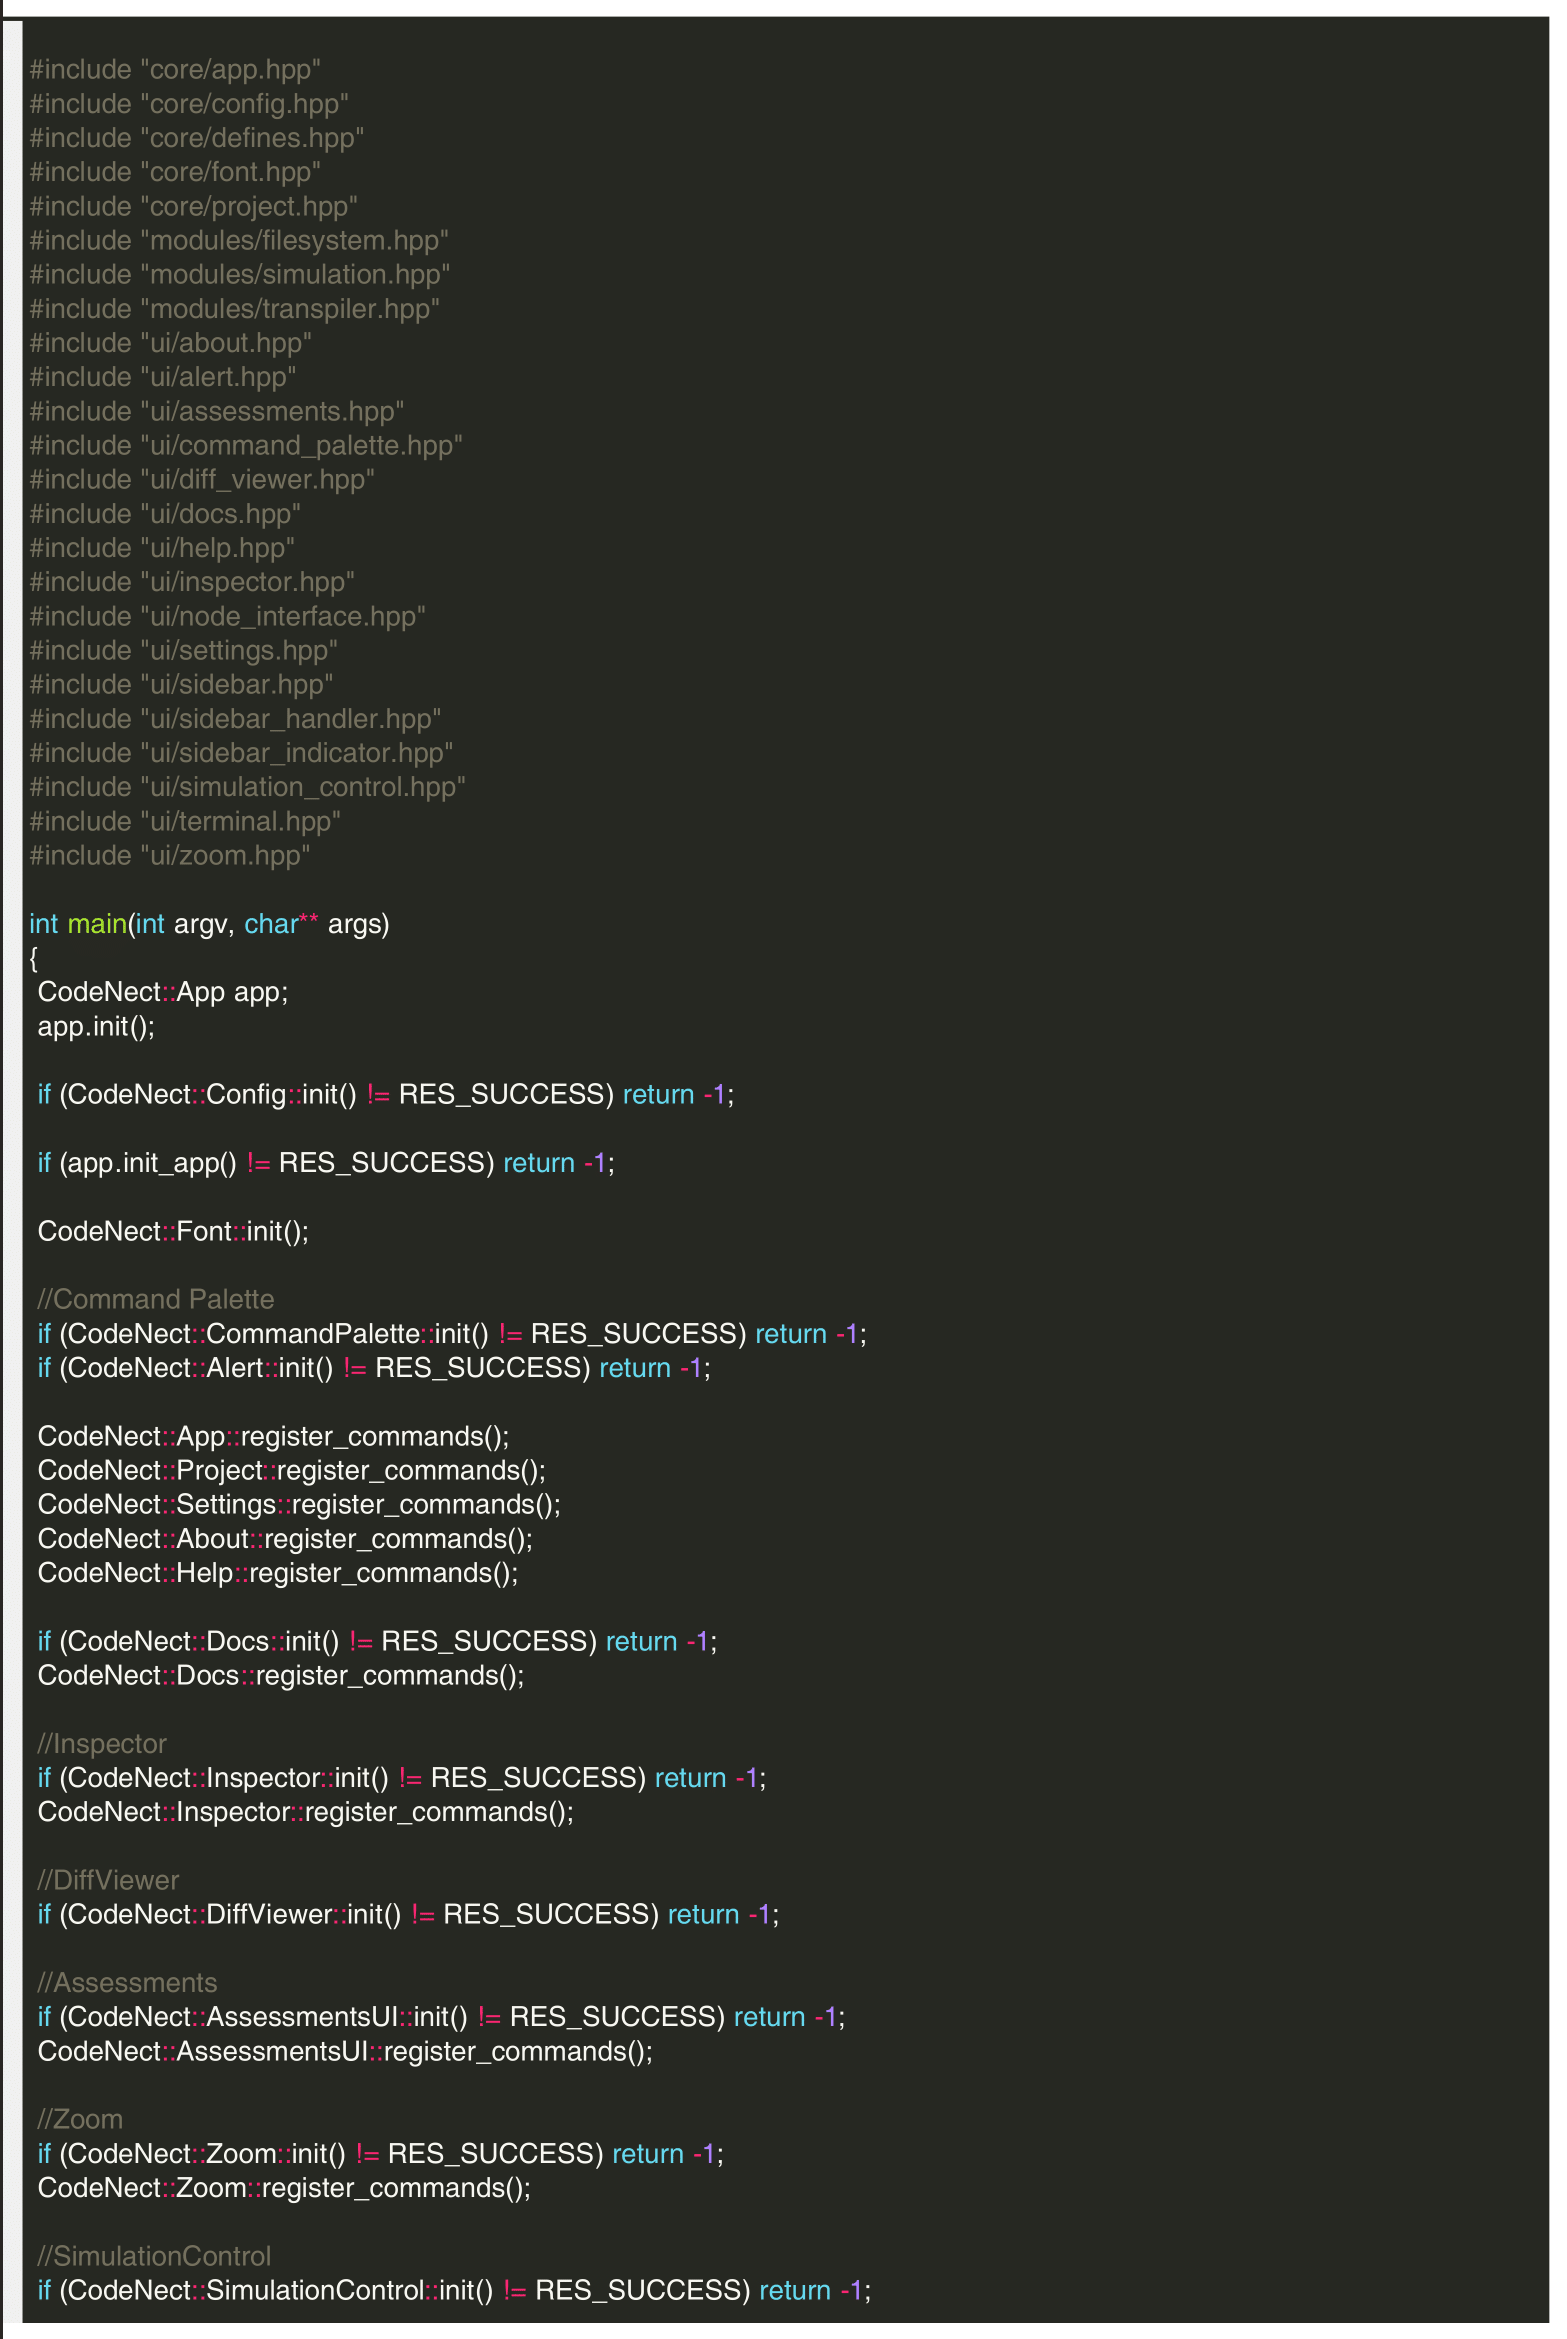
\includegraphics[width=\textwidth]{figures/code/main-1.png}
\end{figure}
\begin{figure}[H]
	 \centering
	 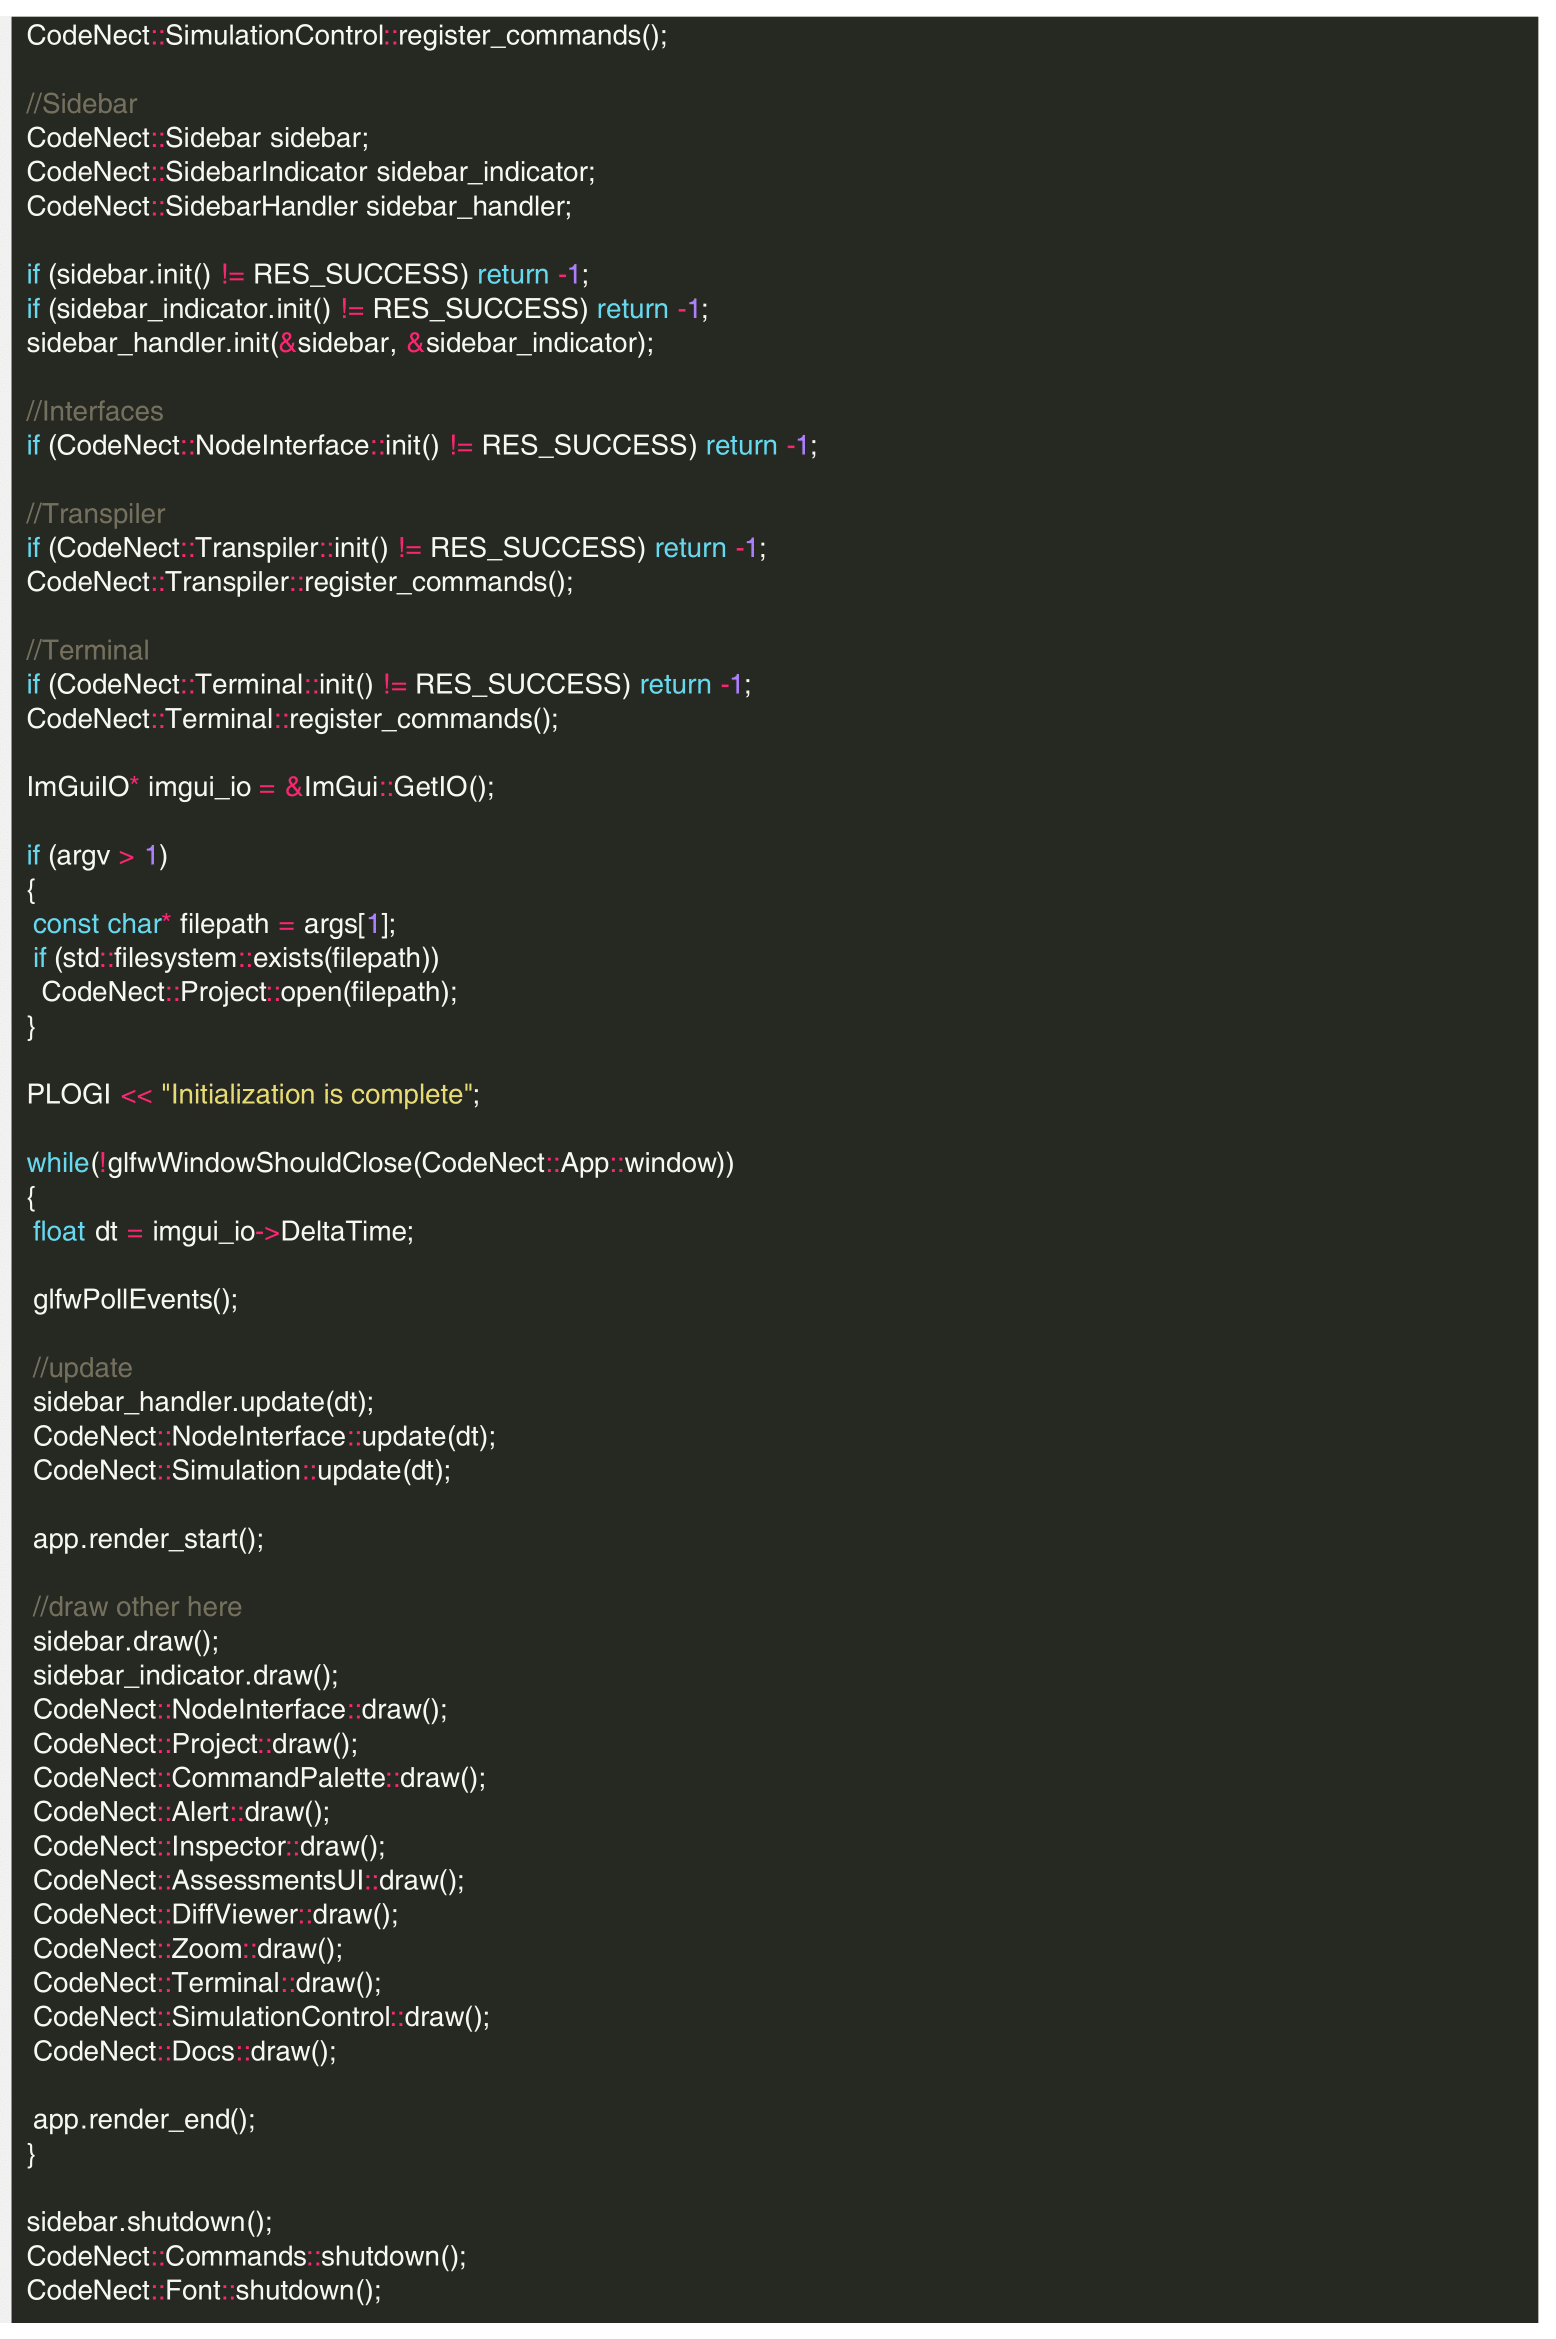
\includegraphics[width=\textwidth]{figures/code/main-2.png}
\end{figure}
\begin{figure}[H]
	 \centering
	 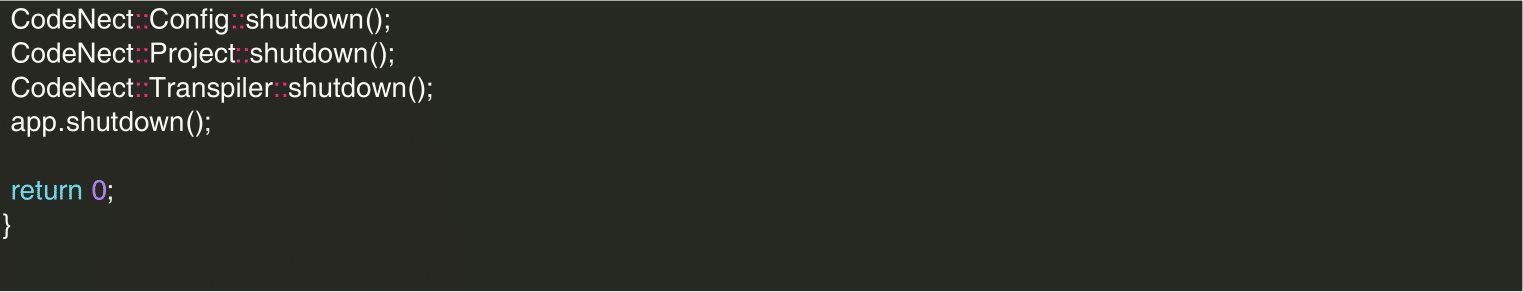
\includegraphics[width=\textwidth]{figures/code/main-3.png}
\end{figure}

\begin{figure}[H]
	 \centering
	 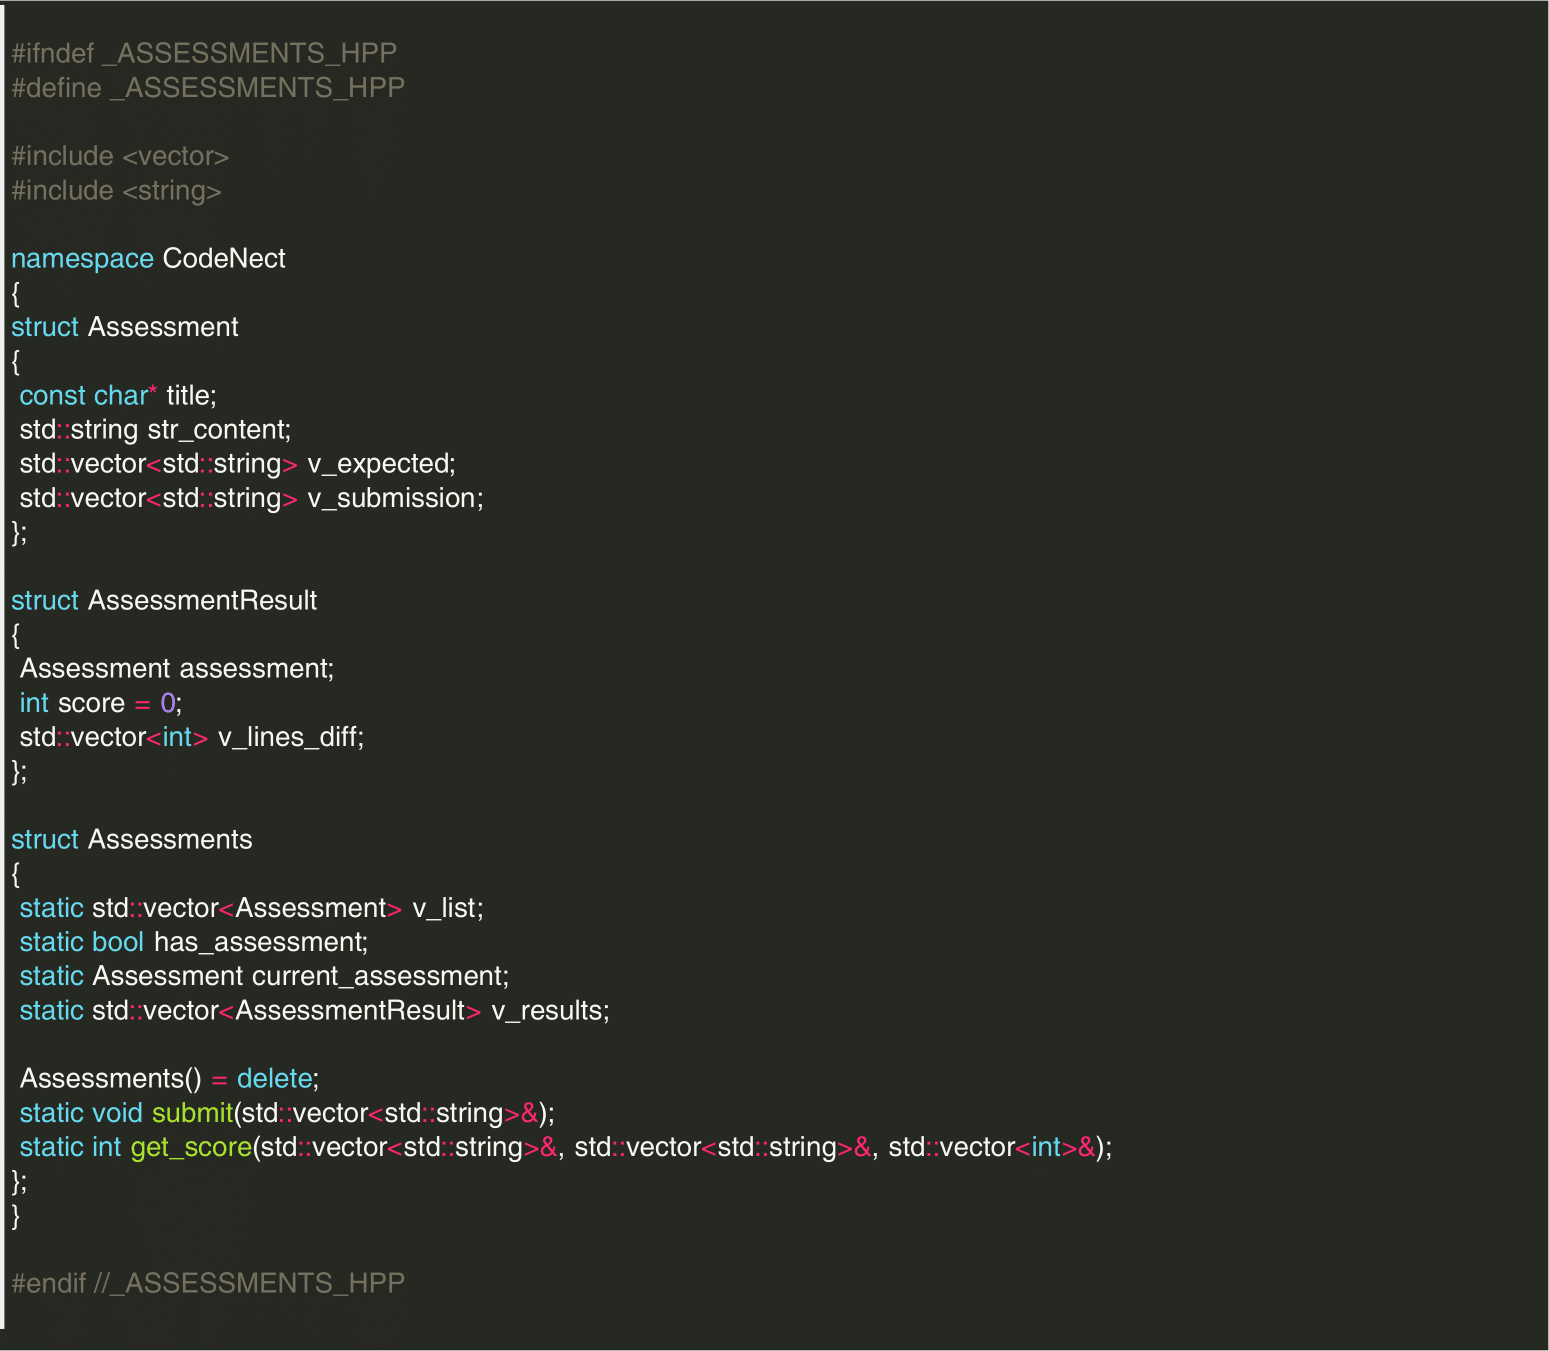
\includegraphics[width=\textwidth]{figures/code/assessments.png}
\end{figure}
\begin{figure}[H]
	 \centering
	 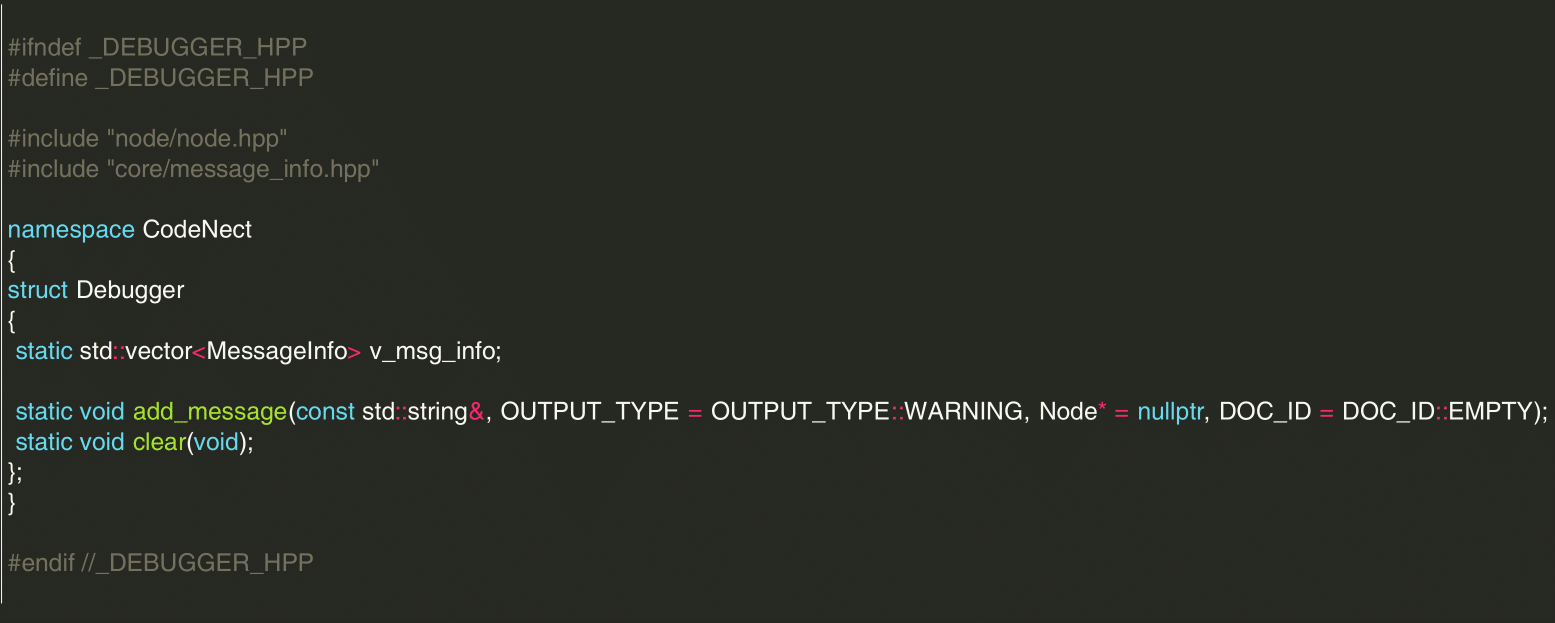
\includegraphics[width=\textwidth]{figures/code/debugger.png}
\end{figure}
\begin{figure}[H]
	 \centering
	 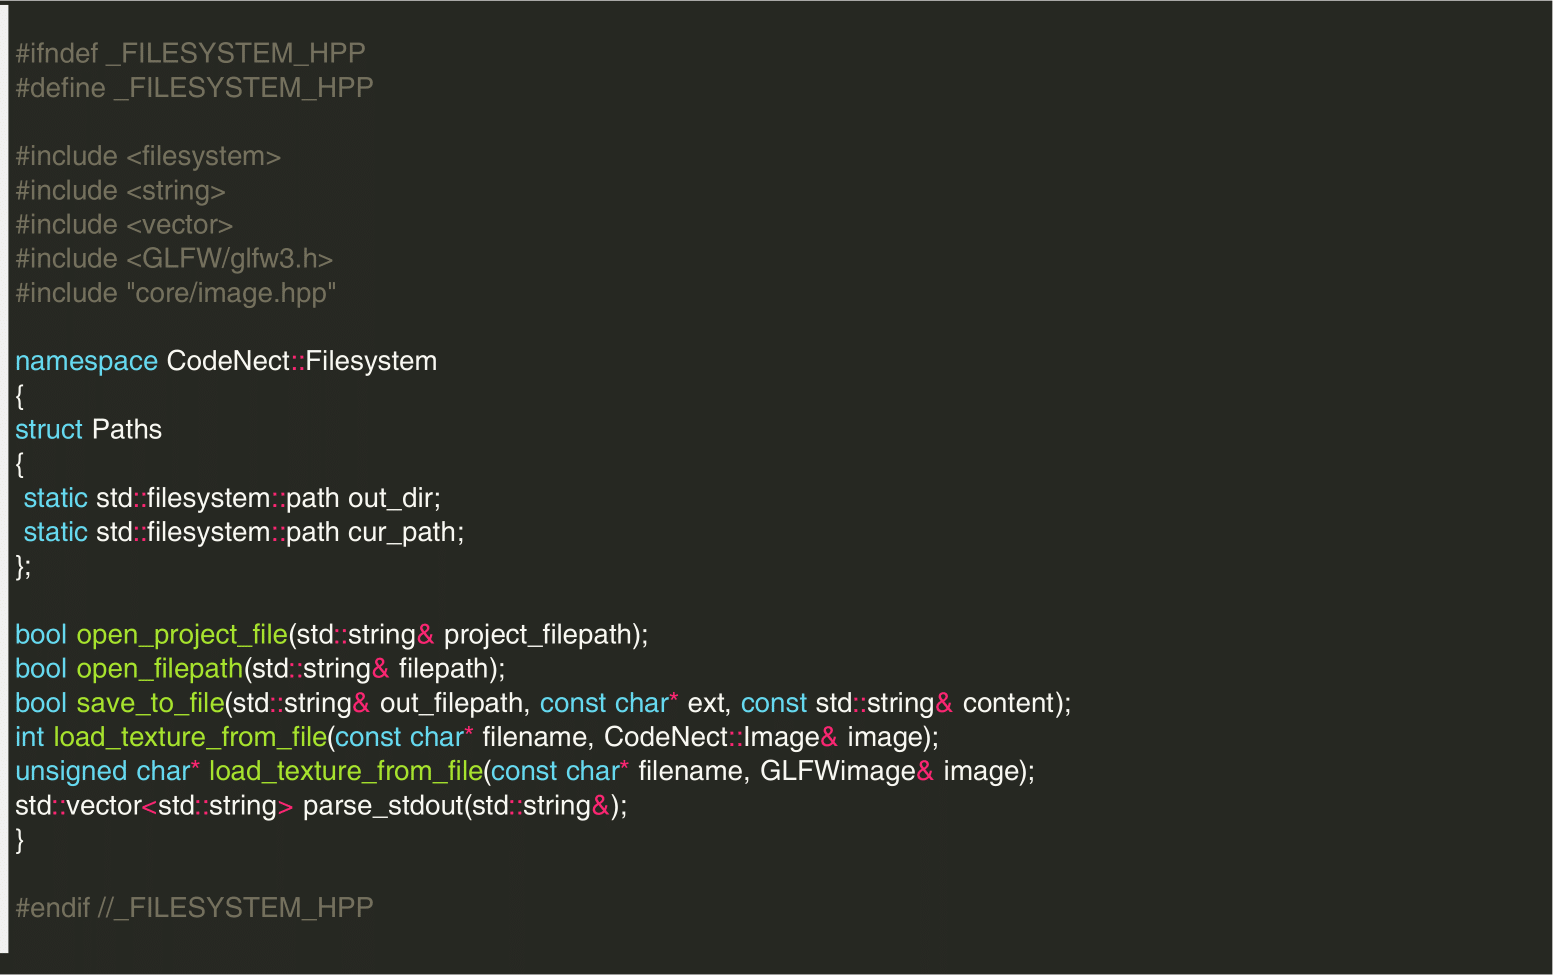
\includegraphics[width=\textwidth]{figures/code/filesystem.png}
\end{figure}
\begin{figure}[H]
	 \centering
	 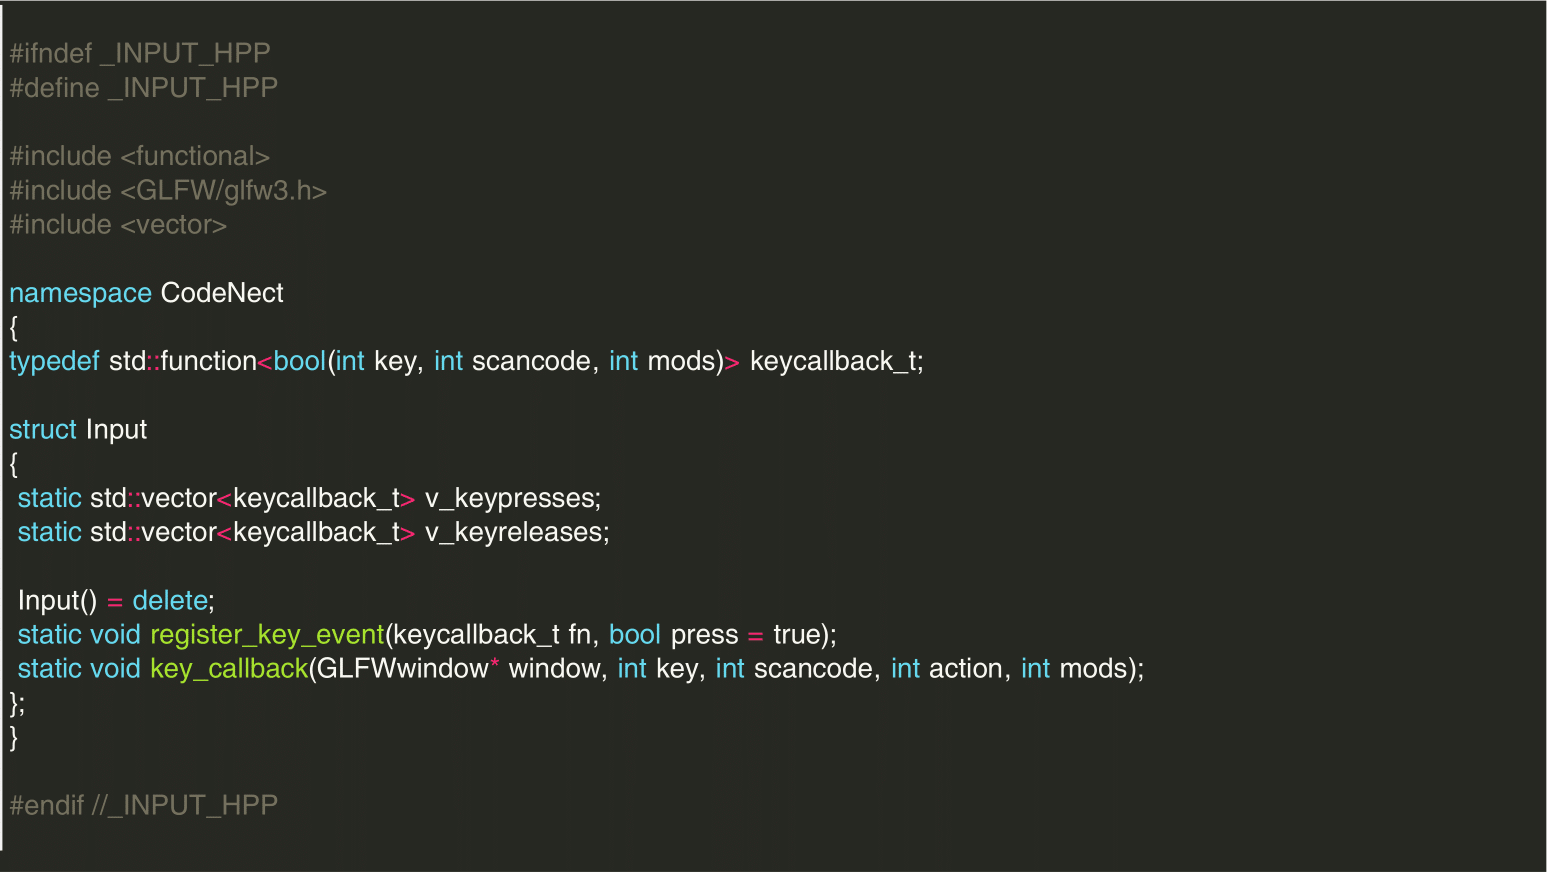
\includegraphics[width=\textwidth]{figures/code/input.png}
\end{figure}
\begin{figure}[H]
	 \centering
	 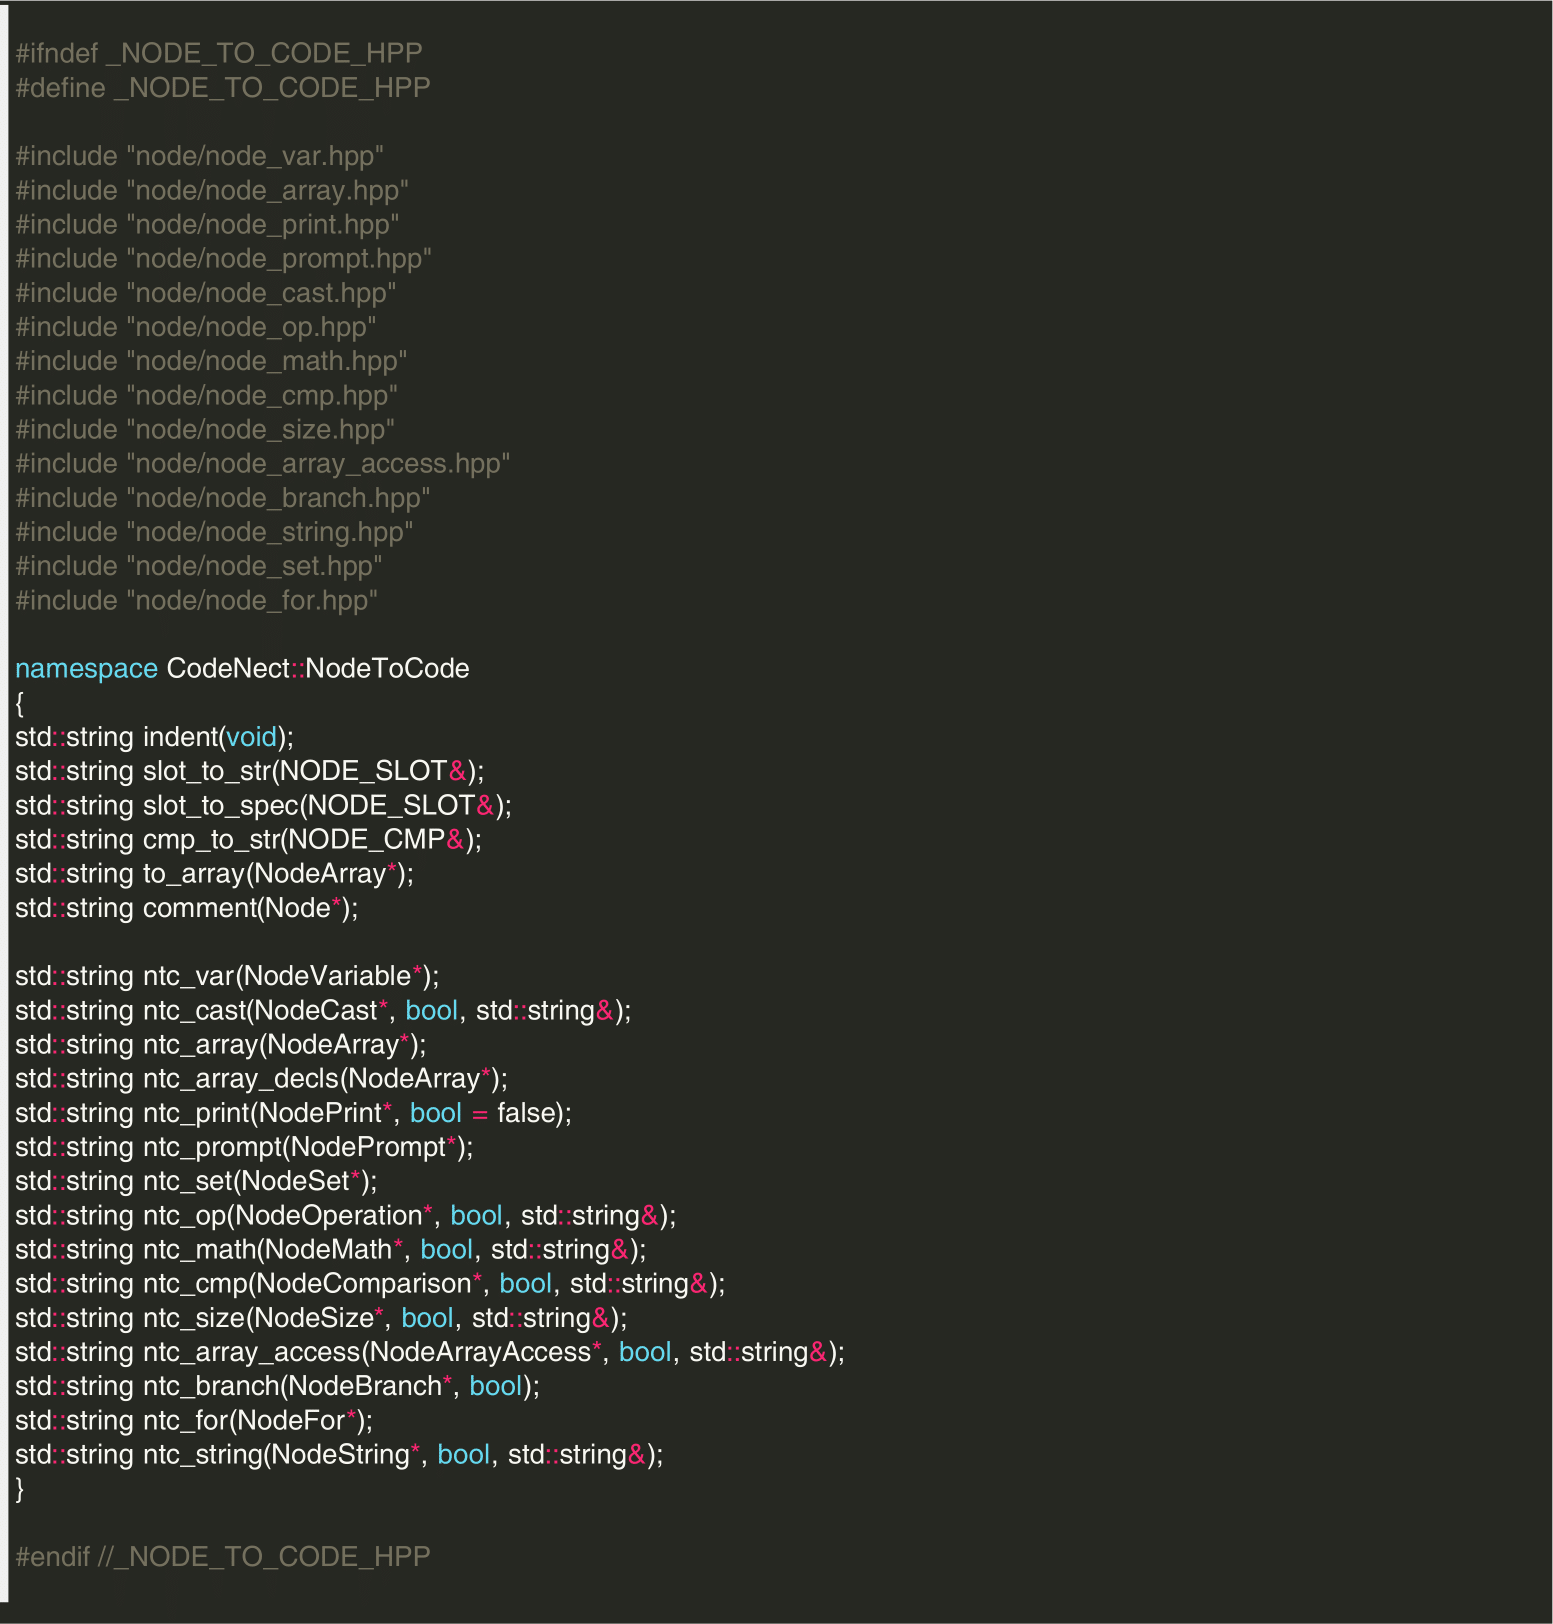
\includegraphics[width=\textwidth]{figures/code/node_to_code.png}
\end{figure}
\begin{figure}[H]
	 \centering
	 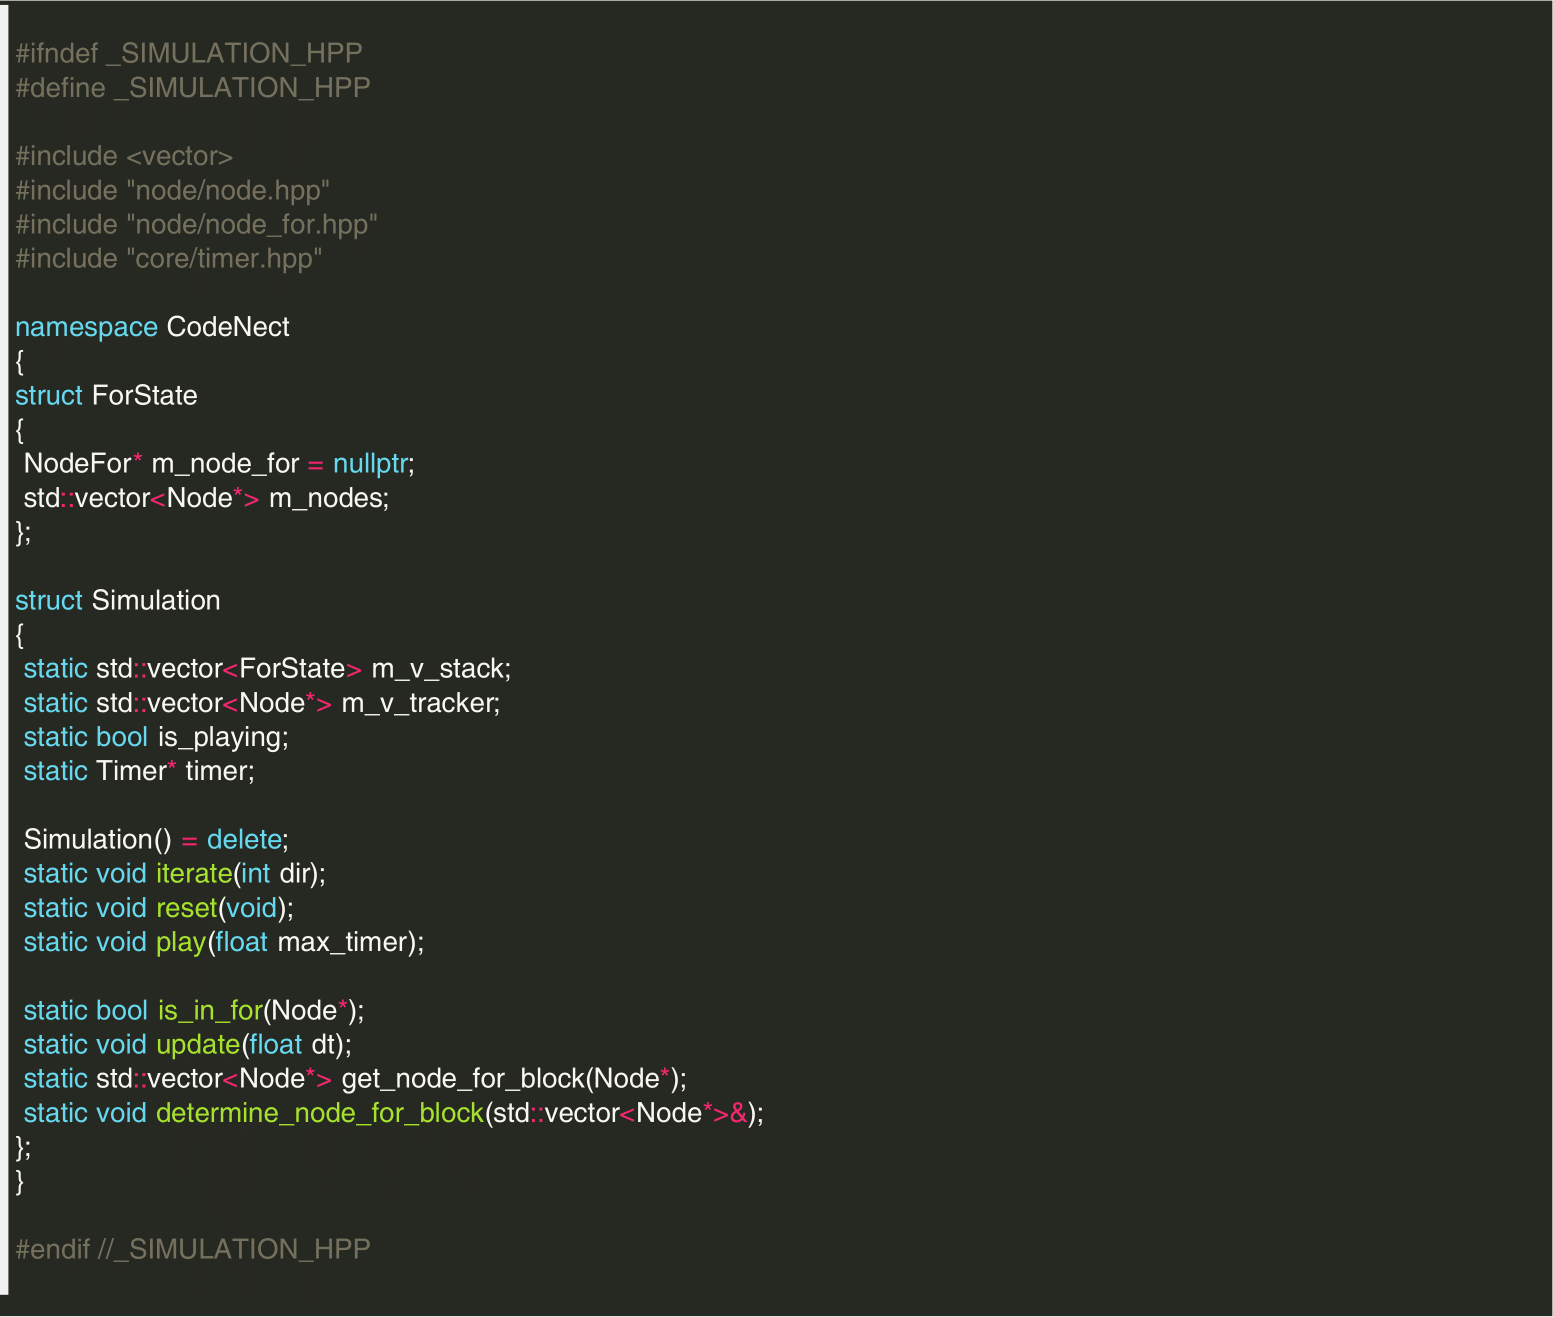
\includegraphics[width=\textwidth]{figures/code/simulation.png}
\end{figure}
\begin{figure}[H]
	 \centering
	 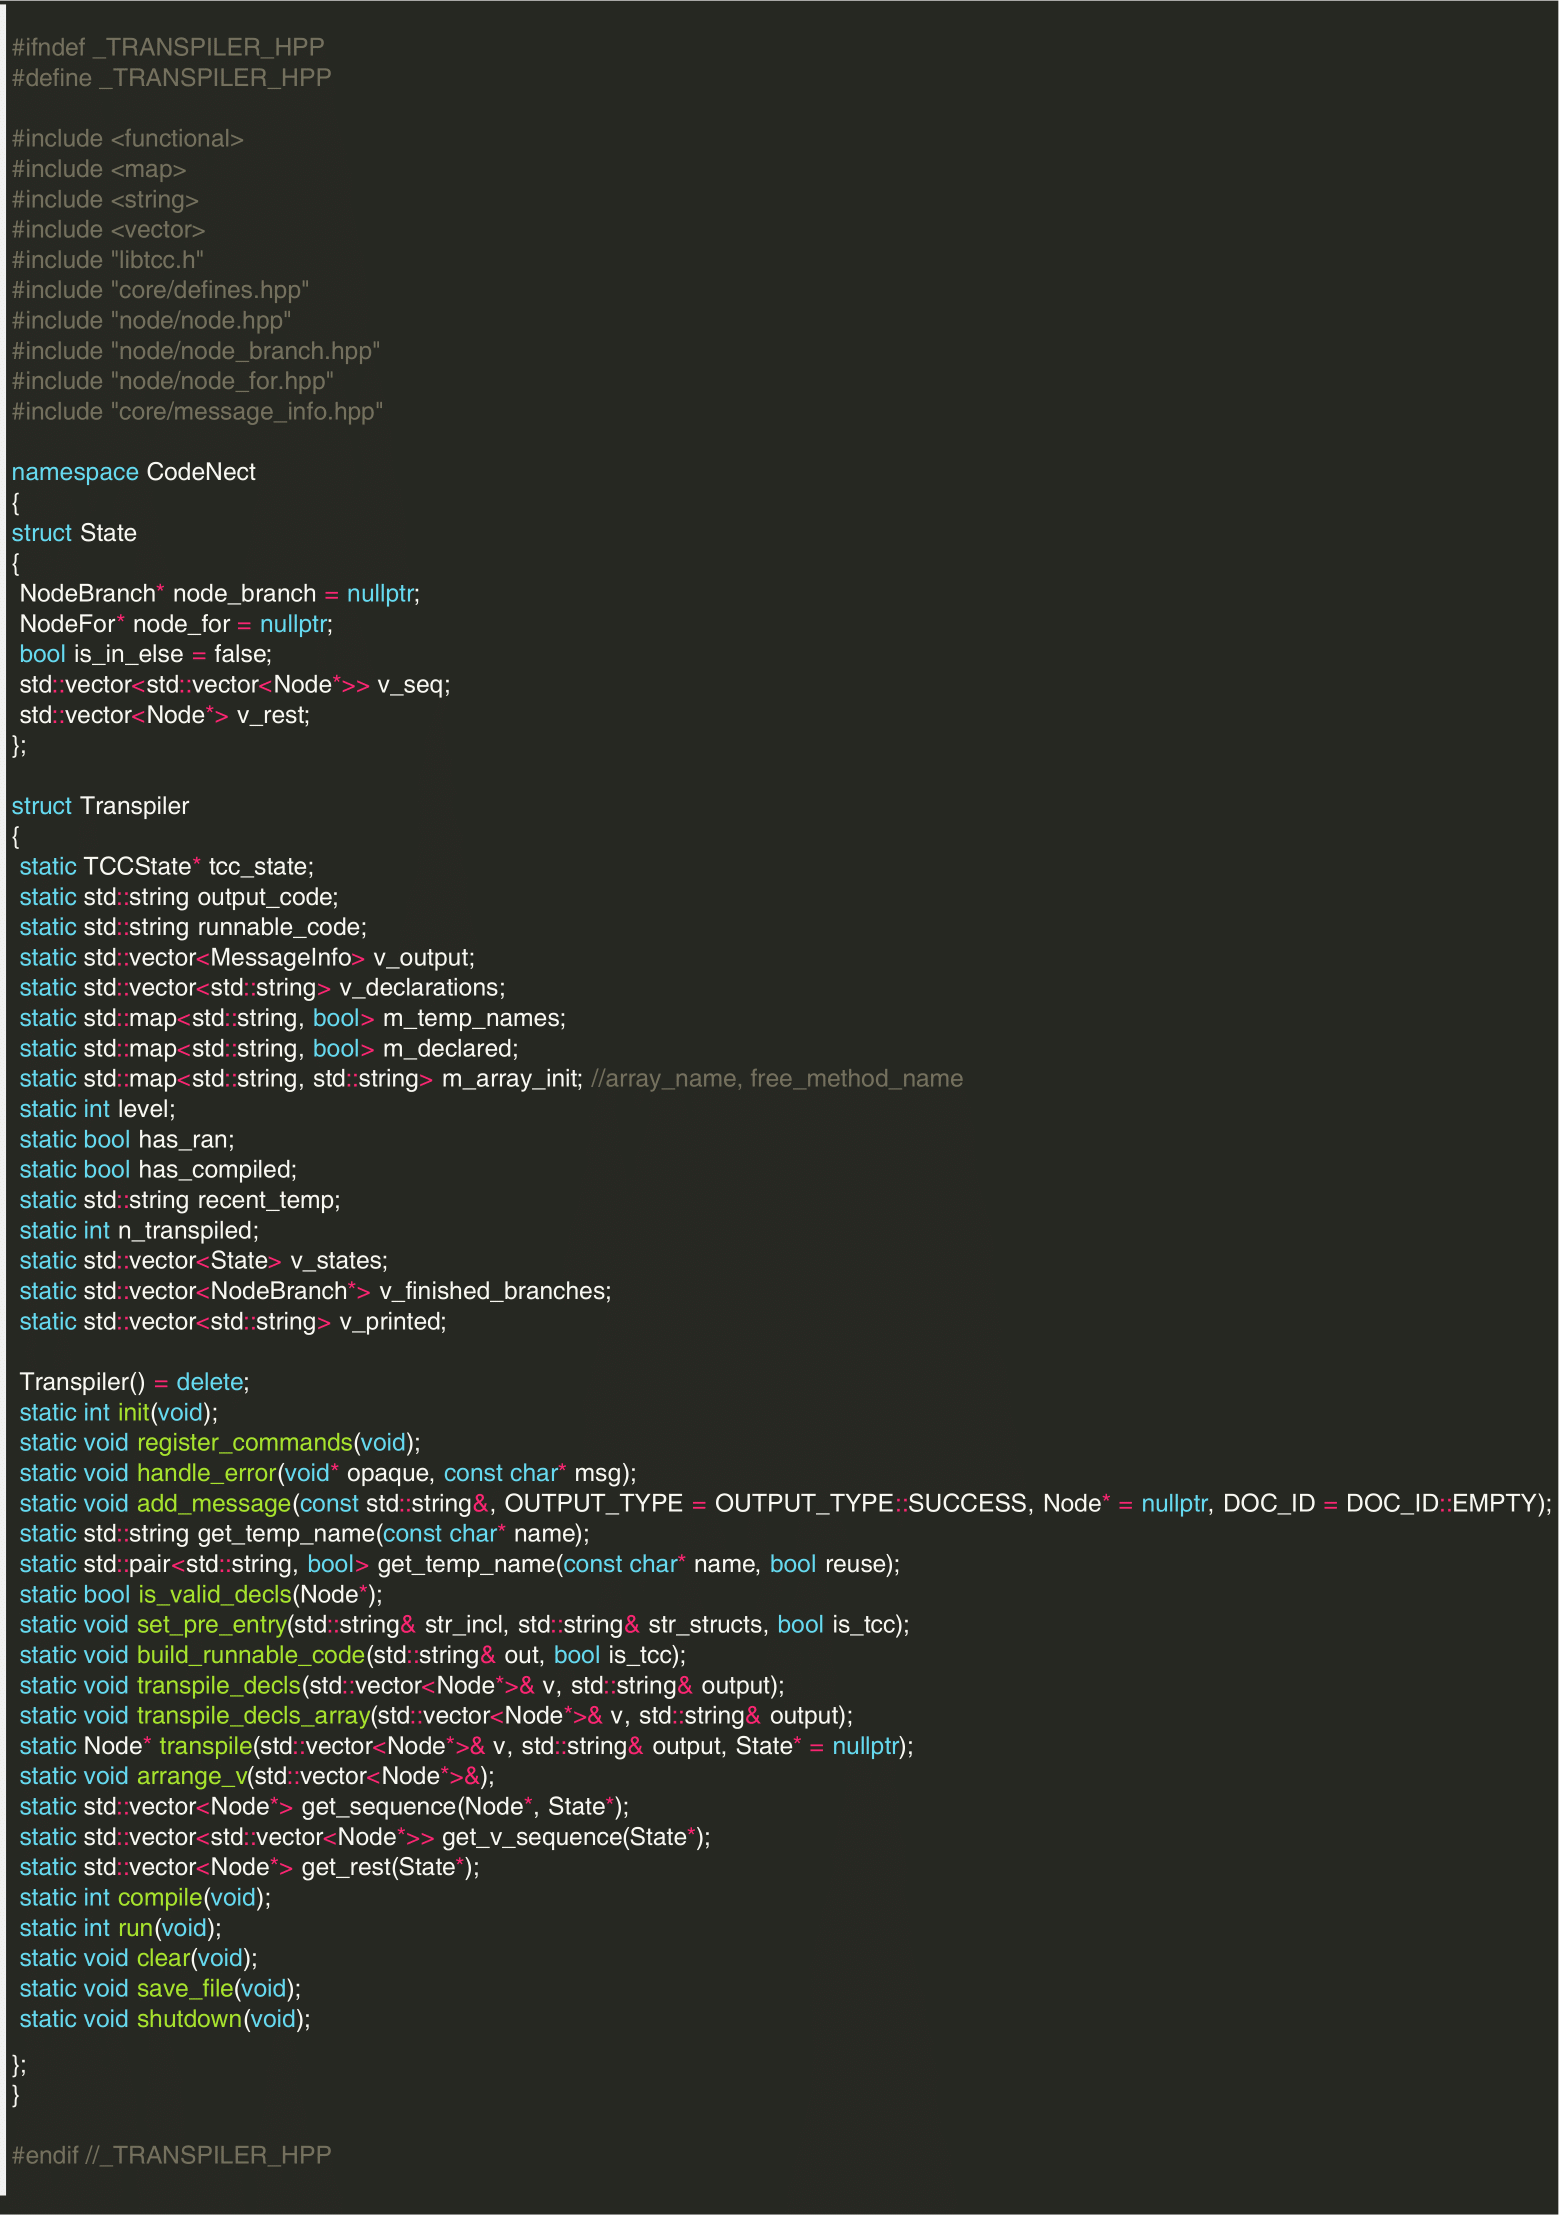
\includegraphics[width=\textwidth]{figures/code/transpiler.png}
\end{figure}
